\section{Model3DDyn  Class Reference}
\label{classModel3DDyn}\index{Model3DDyn@{Model3DDyn}}
A spacecraft model with three thrusters providing both tranlation force and rotation torque. 


{\tt \#include $<$model3ddyn.h$>$}

Inheritance diagram for Model3DDyn::\begin{figure}[H]
\begin{center}
\leavevmode
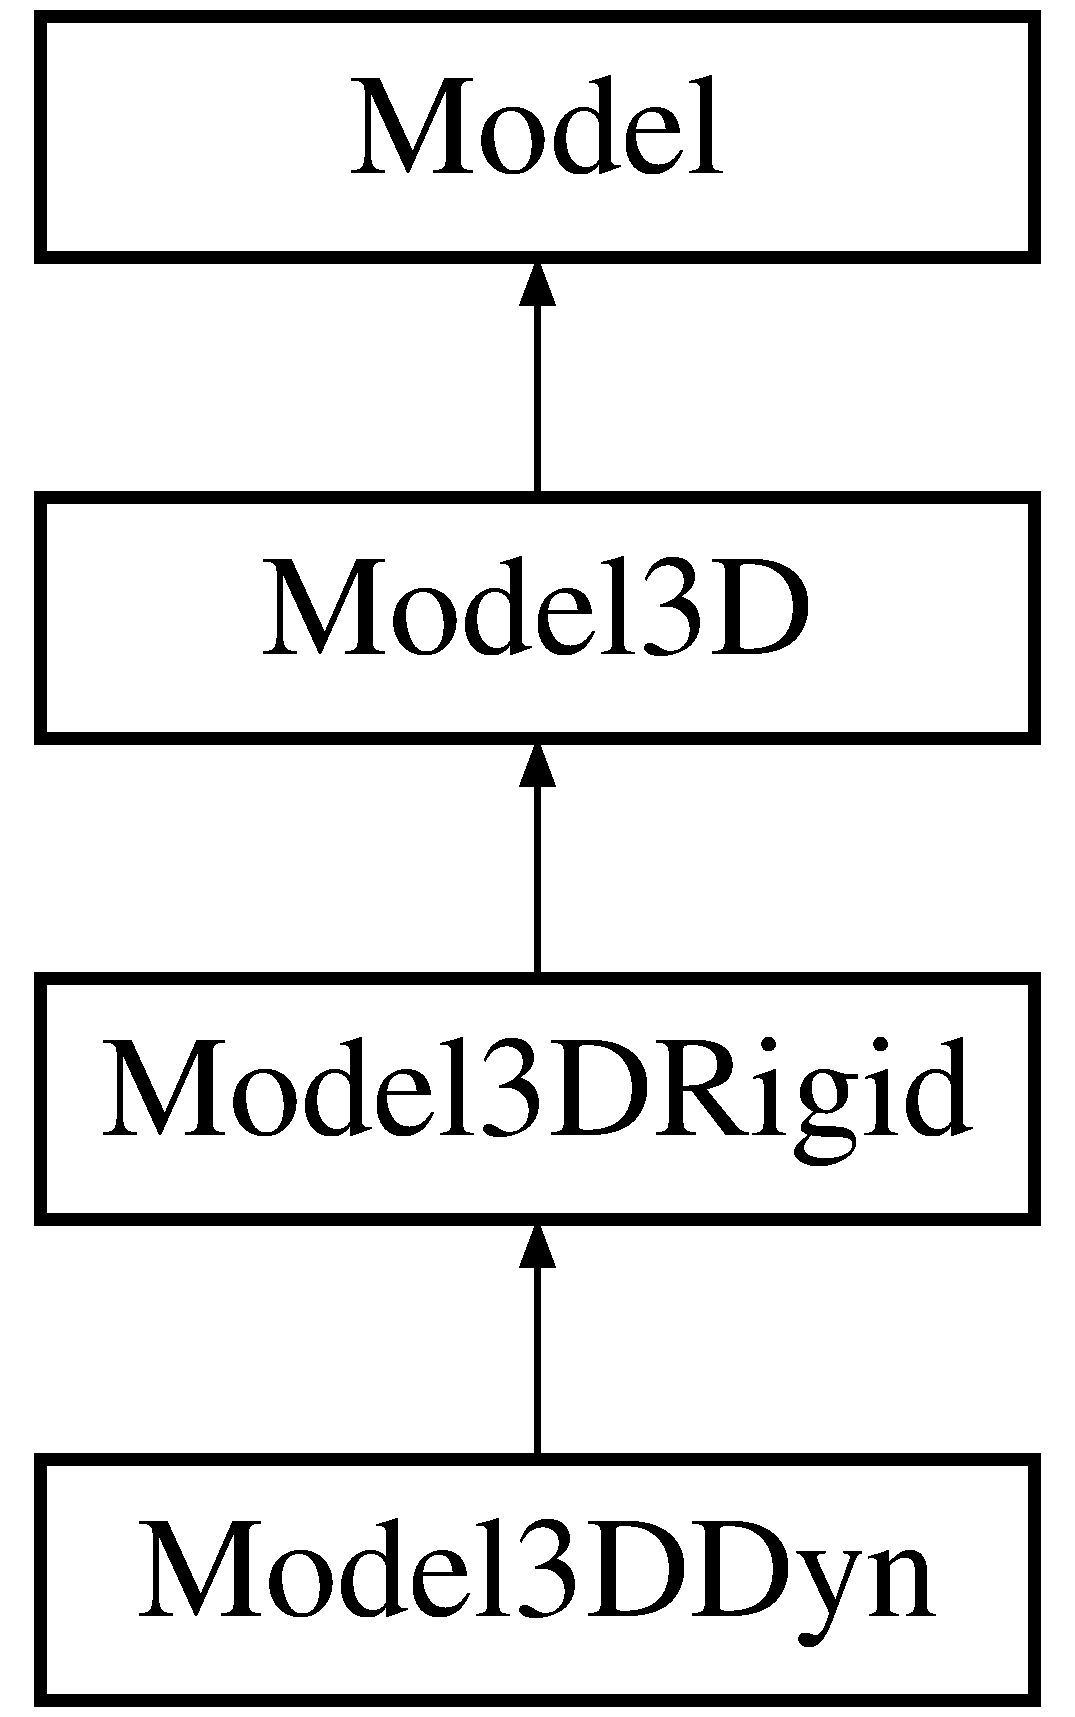
\includegraphics[height=4cm]{classModel3DDyn}
\end{center}
\end{figure}
\subsection*{Public Methods}
\begin{CompactItemize}
\item 
{\bf Model3DDyn} (string path)
\item 
virtual {\bf $\sim$Model3DDyn} ()
\item 
virtual {\bf MSLVector} {\bf State\-Transition\-Equation} (const {\bf MSLVector} \&x, const {\bf MSLVector} \&u)
\begin{CompactList}\small\item\em The state transition equation, or equations of motion, xdot=f(x,u).\item\end{CompactList}\item 
virtual bool {\bf Satisfied} (const {\bf MSLVector} \&state)
\begin{CompactList}\small\item\em Test whether global state-space constraints are satisfied.\item\end{CompactList}\end{CompactItemize}
\subsection*{Public Attributes}
\begin{CompactItemize}
\item 
double {\bf m}
\item 
{\bf MSLMatrix} {\bf I}
\end{CompactItemize}


\subsection{Detailed Description}
A spacecraft model with three thrusters providing both tranlation force and rotation torque.



\subsection{Constructor \& Destructor Documentation}
\index{Model3DDyn@{Model3DDyn}!Model3DDyn@{Model3DDyn}}
\index{Model3DDyn@{Model3DDyn}!Model3DDyn@{Model3DDyn}}
\subsubsection{\setlength{\rightskip}{0pt plus 5cm}Model3DDyn::Model3DDyn (string {\em path} = \char`\"{}\char`\"{})}\label{classModel3DDyn_a0}


\index{Model3DDyn@{Model3DDyn}!~Model3DDyn@{$\sim$Model3DDyn}}
\index{~Model3DDyn@{$\sim$Model3DDyn}!Model3DDyn@{Model3DDyn}}
\subsubsection{\setlength{\rightskip}{0pt plus 5cm}Model3DDyn::$\sim$Model3DDyn ()\hspace{0.3cm}{\tt  [inline, virtual]}}\label{classModel3DDyn_a1}




\subsection{Member Function Documentation}
\index{Model3DDyn@{Model3DDyn}!Satisfied@{Satisfied}}
\index{Satisfied@{Satisfied}!Model3DDyn@{Model3DDyn}}
\subsubsection{\setlength{\rightskip}{0pt plus 5cm}bool Model3DDyn::Satisfied (const {\bf MSLVector} \& {\em state})\hspace{0.3cm}{\tt  [virtual]}}\label{classModel3DDyn_a3}


Test whether global state-space constraints are satisfied.



Reimplemented from {\bf Model} {\rm (p.\,\pageref{classModel_a4})}.\index{Model3DDyn@{Model3DDyn}!StateTransitionEquation@{StateTransitionEquation}}
\index{StateTransitionEquation@{StateTransitionEquation}!Model3DDyn@{Model3DDyn}}
\subsubsection{\setlength{\rightskip}{0pt plus 5cm}{\bf MSLVector} Model3DDyn::State\-Transition\-Equation (const {\bf MSLVector} \& {\em x}, const {\bf MSLVector} \& {\em u})\hspace{0.3cm}{\tt  [virtual]}}\label{classModel3DDyn_a2}


The state transition equation, or equations of motion, xdot=f(x,u).



Reimplemented from {\bf Model3DRigid} {\rm (p.\,\pageref{classModel3DRigid_a3})}.

\subsection{Member Data Documentation}
\index{Model3DDyn@{Model3DDyn}!I@{I}}
\index{I@{I}!Model3DDyn@{Model3DDyn}}
\subsubsection{\setlength{\rightskip}{0pt plus 5cm}{\bf MSLMatrix} Model3DDyn::I}\label{classModel3DDyn_m1}


\index{Model3DDyn@{Model3DDyn}!m@{m}}
\index{m@{m}!Model3DDyn@{Model3DDyn}}
\subsubsection{\setlength{\rightskip}{0pt plus 5cm}double Model3DDyn::m}\label{classModel3DDyn_m0}




The documentation for this class was generated from the following files:\begin{CompactItemize}
\item 
{\bf model3ddyn.h}\item 
{\bf model3ddyn.C}\end{CompactItemize}
